\section{Methodology}
\label{sec:methodology}

A systematic literature review uses explicit, rigorous, and reproducible systematic methods to synthesize the findings of studies related to a particular research question, topic area, or phenomenon of interest. This type of review assures the quality and trustworthiness of the review's findings by presenting a complete, organized, and summarized analysis of all works considered while allowing others to replicate or update the reviews. The most common standard for performing a systematic review is the PRISMA~\parencite{methodology:prisma} statement. Although the PRISMA statement has been designed originally for evaluating the effects of health interventions, the checklist items of the methodology are general and applicable to other subject areas. Thus, the methodology used in this systematic review follows the PRISMA~\parencite{methodology:prisma} guidelines.

This section presents the detailed methodology used in this study. First, the eligibility criteria decide which studies to include in the review. Next, the search strategy details the information sources considered in the review and the base string and search fields used for inquiring these sources. Furthermore, the selection process focuses on describing its stages and the quality evaluation criteria used to select works for the synthesis and analysis phase of the review. Lastly, the data extraction process details the relevant data collected for synthesis and analysis.
Parsifal \parencite{methodology:parsifal} is the online tool used to support the literature review in designing the methodology protocol, removing duplicates, screening and selecting works including their quality assessment. Additional documentation and scripts developed within the scope of this review related to removing duplicates, checking and processing the bibliographic references, and data extraction are available in the public GitHub repository.

\subsection{Eligibility criteria}
\label{sec:methodology:eligible}

Table~\ref{tab:methodology:exclusion-criteria} presents the exclusion criteria used to determine the eligible studies for the selection process. These eligibility criteria focus mainly on the type of paper and availability. The index criterion rejects all publications not indexed in a scientific publication venue. This rejection guarantees that the eligible works were peer-reviewed by the scientific community. Also, the exclusion criteria reject short papers and gray, secondary, and tertiary literature. Short papers do not usually present a detailed methodology of their scientific contribution. As for only considering primary literature in the review, this criterion increases the relevance of search results by favoring original articles and simultaneously guaranteeing peer-revision of the works. In terms of language, only considering studies with English full-texts increases the scope and visibility of the review. Similarly, the eligibility criteria reject studies not available in digital libraries for reproducibility and accessibility reasons.

\begin{table}[h]
  \renewcommand{\arraystretch}{1.25}
  \setlength{\tabcolsep}{3pt}
  \caption[Exclusion criteria for the selection process.]{Exclusion criteria for the selection process.}
  \label{tab:methodology:exclusion-criteria}
  \centering
  {\scriptsize
  \begin{tabular}{c m{0.28\columnwidth} m{0.6\columnwidth}}

\hline
\textbf{E\#} & \textbf{Criteria} & \textbf{Statement}\\
\hline
E1 &
Index &
Papers not indexed in a scientific publication venue\\
\hline
E2 &
Language &
Full-text of the papers not published in English\\
\hline
E3 &
Subject Area &
Papers not classified in the databases as Computer Science, Engineering, Mathematics, or Multidisciplinary\\
\hline
E4 &
Short Papers &
Papers classified as short papers accordingly to the publication venue\\
\hline
E5 &
Gray, Secondary, and Tertiary Literature &
Books, preprints, reports, reviews, thesis, ...\\
\hline
E6 &
Availability &
Full-text of the papers not available in digital libraries\\
\hline
E7 &
Dataset &
Papers that focus only on data collection\\
\hline
E8 &
Coverage &
Papers using only odometry for localization\\
\hline
E9 &
Scope &
Papers that focus on different and not related subjects\\
\hline

  \end{tabular}}
\end{table}

Another exclusion criterion considered in the review is relative to the studies' categorization of their subject areas by bibliographic databases. The ones considered in the review are Computer Science, Engineering, Mathematics, or Multidisciplinary areas. In the list provided by the Clarivate's Journal Citation Reports\footnote{\url{https://jcr.clarivate.com/jcr/browse-categories}}, these four subject areas include the artificial intelligence, interdisciplinary applications, electrical and computers engineering, robotics, and applied mathematics categories, among others. These categories are intrinsically related to the localization and mapping problem for long-term operation of mobile robots.

The final three criteria presented in Table~\ref{tab:methodology:exclusion-criteria} focus on the scientific contribution of the studies. The dataset criterion rejects all works that focus only on sharing a data collection. Although these works are important for the evolution of localization and mapping algorithms in providing a benchmark for comparison and reference purposes, their scientific contribution is not directly comparable to research articles. Odometry-only approaches are unusable over long distances invalidating their use for long-term operations with mobile robots. As for the scope criterion, this review does not consider as eligible papers not related to long-term localization and mapping that do not fall under the other exclusion criteria.

\subsection{Search strategy}
\label{sec:methodology:search}

The search phase consists of identifying the data sources that could be relevant for this literature review, and defining the base string and which search fields considered to obtain the results for the review. \citetitle{methodology:search:db:wos} and \citetitle{methodology:search:db:scopus} are traditionally the two most widely used bibliographic databases. However, previous studies demonstrate that different databases differ significantly in their scientific coverage~\parencite{methodology:search:db:coverage:scopus-wos,methodology:search:db:coverage:dim-scopus-wos}. Thus, the data sources considered in this review are the following ones: \citetitle{methodology:search:db:acm}, \citetitle{methodology:search:db:dimensions}, \citetitle{methodology:search:db:ieee-xplore}, \citetitle{methodology:search:db:inspec}, \citetitle{methodology:search:db:scopus}, and \citetitle{methodology:search:db:wos}.

Moreover, May 17, 2022, is the date of the last full inquiry. Future reviews on the topic of this study should consider this final date as theirs initial one. As for inquiring the data sources, the base string used is the following one:

\vspace{1em}

\noindent\begin{center}
\begin{tabular}{l l}
\texttt{(robot* OR vehicle*)}                     & \texttt{AND}\\
\texttt{((locali* AND map*) OR "slam")}           & \texttt{AND}\\
\texttt{("long term" OR "life long" OR lifelong)}\\
\end{tabular}
\end{center}

\vspace{1em}

The first terms, \texttt{robot* OR vehicle*}, attempt to focus the search results to the desired population. These two terms have multiple synonyms within the scope of autonomous mobile robots: mobile robots, autonomous vehicles, robotics, agricultural robots, intelligent robots, service robots, unmanned aerial/ground/underwater vehicles, among other terms. Therefore, by adding the asterisk to the end of the terms robot and vehicle (\texttt{robot*} and \texttt{vehicle*}, respectively), and by only considering the terms with asterisk in the inquiry, all the synonyms are covered for the desired population. Given the incompatibility of the \citetitle{methodology:search:db:dimensions} database with wildcards (e.g., using the asterisk), the first part of the base string becomes as follows when searching in this database: \texttt{robot OR robots OR robotics OR vehicle OR vehicles}.

The next part of the query focus on the intervention side of the systematic review. Given the interest of this review on searching for localization and mapping algorithms, \texttt{locali*} and \texttt{map*} summarize all the synonyms for the localization and mapping terms, respectively. For example, \texttt{locali*} not only is agnostic to the US versus UK spelling differences (localization vs localisation, respectively) but also resumes several synonyms: localization, localize, or localizing. The term \texttt{map*} also attempts to cover its respective synonyms such as map, maps, or mapping.
Also, the acronym \texttt{"slam"} is another alternative to search for localization and mapping algorithms. Even though its definition is compatible with \texttt{locali* AND map*}, some authors only refer to SLAM.
Similarly to the inquiry's first part, the second one becomes as follows for searching in \citetitle{methodology:search:db:dimensions}: \texttt{((localize OR localization OR localizing OR localise OR localisation OR localising) AND (map OR maps OR mapping)) OR "slam"}.

As for \texttt{"long term" OR "life long" OR lifelong}, this part of the base string is relative to the outcome of the PICO framework, presented in Section~\ref{sec:purpose}. The reason for having both \texttt{"life long"} and \texttt{lifelong} terms is the existing confusion in which term is grammatically the correct one.

Furthermore, the Title, Abstract, and Keywords are the fields considered for obtaining the search results. The third one includes the author keywords, the indexed terms by the databases, and the uncontrolled ones if they are available. The selection of these search fields for this review improves the relevance of the results compared to using all fields and the full text by focusing the search on the summary items of the works. Indeed, the main contributions of scientific works should be summarized in at least the title, abstract, or the author keywords. The indexed terms also help in obtaining records only related to the base string used in this review.
However, not all data sources have available the search fields considered in the review or some of them require an adaptation when performing the search. 
Although the \citetitle{methodology:search:db:acm} allows searching within multiple search fields, including the ones considered in this review, the advanced search query on this library sets by default an AND operator between the different fields. This setting must be changed manually in the query syntax to the desired OR operator. Also, there are two options to search items in the \citetitle{methodology:search:db:acm}: \textit{The ACM Full-Text Collection} and \textit{The ACM Guide to Computing Literature}. Given that the latter includes all the content from the former, the identification process in this source performs the search using \textit{The ACM Guide to Computing Literature} option.
Other than searching in the publications' full data, \citetitle{methodology:search:db:dimensions} only has the title and abstract search fields compatible with this review. Given the limitation of \citetitle{methodology:search:db:ieee-xplore} to 7 wildcards, the search results of this digital library using the base string for the inquiry are the grouping of different searches considering only a search field at a time, importing each search results to Parsifal and removing the duplicates. As for \citetitle{methodology:search:db:inspec}, \citetitle{methodology:search:db:scopus}, and \citetitle{methodology:search:db:wos}, these databases have available all the search fields considered in the review.

In terms of the publication date, this review does not restrict it to avoid ignoring important works and to improve the discussion. Indeed, to best of the authors knowledge, there is not available a systematic review on long-term localization and mapping for mobile robots to provide an initial date for rejecting older publications. Even though the number of publications per year could indicate an initial date on when the topic gained relevance, the date filtering could still reject important works.

\subsection{Selection process}
\label{sec:methodology:selection}

The selection process of this review summarized in Figure~\ref{fig:methodology:prisma-flow} has three phases: identification, screening, and quality assessment. The first phase consists of inquiring each data source discussed previously with the base string and adapting it if needed. The second phase requires screening the papers. In this review, screening is equivalent to reading the publications' title and abstract and deciding whether the study is eligible or not based on the exclusion criteria. Then, a set of evaluation criteria assesses the quality of the eligible records. The records obtained after the three phases of the selection process are for the data extraction phase.

\begin{figure}[h]
  \centering
  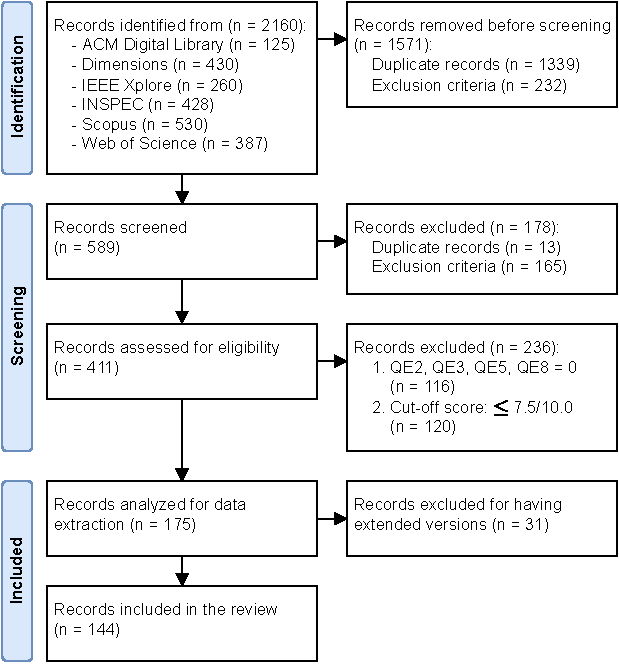
\includegraphics[width=\columnwidth]{figures/selection.pdf}
  \caption{PRISMA flow diagram for the selection process.}
  \label{fig:methodology:prisma-flow}
\end{figure}

\subsubsection{Identification}

In the identification phase of this review, the search strategy is applied to all data sources. \citetitle{methodology:search:db:acm}, \citetitle{methodology:search:db:dimensions}, \citetitle{methodology:search:db:inspec}, \citetitle{methodology:search:db:scopus}, and \citetitle{methodology:search:db:wos} data sources only require a single inquiry to obtain the search results.
Given the limitation of the \citetitle{methodology:search:db:ieee-xplore} for using wildcards mentioned in Section~\ref{sec:methodology:search}, the number of records for this source presented in Figure~\ref{fig:methodology:prisma-flow} represents the results of 7 inquiries (using the fields title, abstract, author keywords, IEEE terms, INSPEC controlled terms, and the INSPEC uncontrolled ones, respectively) after removing the duplicates with the support of Parsifal. Although the total number of search results found is 2160, Parsifal is used to remove duplicates from different data sources, excluding 1339 records. Following the duplicates removal, the exclusion criteria defined in Section~\ref{sec:methodology:search} exclude 232 works from the review. This exclusion is possible due to \citetitle{methodology:search:db:inspec}, \citetitle{methodology:search:db:scopus}, or \citetitle{methodology:search:db:wos} having filters related to the publication's type, subject area, and language.

The works excluded from the search results also include the ones that do not meet the exclusion criteria E4 and E7. For the first one, a Python script available in the GitHub repository of this review searches studies with a number of pages lower or equal to 4. Even though short papers have a maximum number of 3 pages, the papers with 4 pages do not usually present a detailed methodology.
As for the E7 exclusion criterion, some works are possible to remove from the review by searching in their title for the term ``dataset''.
All excluded articles of this review are double-checked to certify if the exclusion criteria are correctly applied. For example, articles published in the Remote Sensing journal from MDPI do not meet the E3 criterion. Indeed, the Journal Citations Reports from Clarivate classifies it by the following categories: Remote Sensing, Geosciences Multidisciplinary, Environmental Sciences, and Imaging Science \& Photographic Technology. However, most search results from this journal found in the identification phase are directly related to the topic of this review and the respective subject areas. Thus, in these cases and in other ones related to the remaining exclusion criteria, the decision is reverted to consider the initially rejected studies for the next phase of the review.

\subsubsection{Screening}

Next, the screening phase in this review consists of reading the title and abstract of the publications and rejecting the ones that meet the exclusion criteria. However, the initially rejected papers have another assessment for validating the exclusion. The analysis of the results and conclusions of these publications considering the exclusion criteria either confirms the exclusion decision or reverses it to eligible works for quality assessment. As a result of the screening phase, 178 studies are rejected from the initial identified 589 works. The duplicate records found in screening and removed manually are due to titles with invalid characters originated by exporting the search results from the \citetitle{methodology:search:db:dimensions}~database.

\subsubsection{Quality assessment}

The quality evaluation in this review of the selected works from screening follows the 8 Quality Evaluation (QE) criteria presented in Table~\ref{tab:methodology:quality-assessment}. All of them are subjective criteria derived from the analysis of the eligible works. The score column establishes the possible values for the QE criteria, in which the minimum, intermediate, and maximum values correspond to none, partial, and full compliance, respectively.
Furthermore, QE1, QE2, QE4, and QE8 focus on the details provided in the papers, specifically, if the discussion of the related work, the proposed methodology, the experimental setup, and the results are detailed and thoroughly analyzed in the publication, respectively.
The possible scores for QE3 are twice the value of QE1, QE2, QE4, and QE8 due to this criterion being directly related to the topic of the review. A work focusing on both localization and mapping problems will have a score of 2.0 (full compliance). If the study only focuses on one of these problems or none of them, the scores will be 1.0 or 0.0, i.e., partial or no compliance, respectively.
QE5 evaluates the long-term results of the eligible studies and is either 2.0 (full) or 0.0 (no compliance). This criterion has the same range as QE3 for similar reasons, given the focus of this review on long-term localization and mapping algorithms.
The definition of long-term experiments for assigning full compliance in QE5 is the following one: dynamic changing environments (e.g., dynamic elements or semi-static ones), increasing environments or feature maps in terms of their size, redundant data removal, or varying conditions (e.g., different seasons of the year or lighting conditions).
QE6 and QE7 can only be 1.0 or 0.0. The former criterion intends to highlight works that compare themselves to the state of the art and/or ground-truth data. The latter emphasizes the importance of having available either the implementation of the proposed methodology or the data used in the experiments for other works to be able to compare the proposed methodologies.
Lastly, considering the possible scores for the QE criteria in Table~\ref{tab:methodology:quality-assessment}, each work can only have a  maximum score of 10.0.

\begin{table}[h]
  \renewcommand{\arraystretch}{1.25}
  \setlength{\tabcolsep}{3pt}
  \caption[Quality evaluation criteria and score range.]{Quality evaluation criteria and score range.}
  \label{tab:methodology:quality-assessment}
  \centering
  {\scriptsize
  \begin{tabular}{c m{0.68\columnwidth} c}

\hline
\textbf{QE\#} & \textbf{Criteria} & \textbf{Score}\\
\hline
QE1 &
Does the paper have an updated state of the art on long-term localization and mapping? &
\{0.0, 0.5, 1.0\}\\
\hline
QE2 &
Is the methodology appropriate and detailed? &
\{0.0, 0.5, 1.0\}\\
\hline
QE3 &
Does the methodology consider both localization and mapping problems? &
\{0.0, 1.0, 2.0\}\\
\hline
QE4 &
Is the hardware and/or software used in the experiments detailed? &
\{0.0, 0.5, 1.0\}\\
\hline
QE5 &
Does the paper presents any kind of long-term experimental results? &
\{0.0, 2.0\}\\
\hline
QE6 &
Does the paper presents comparative results with other methods and/or ground-truth data? &
\{0.0, 1.0\}\\
\hline
QE7 &
Does the work's implementation and/or the data used in the experiments are publicly available? &
\{0.0, 1.0\}\\
\hline
QE8 &
Is the discussion of the results and conclusions appropriate and detailed? &
\{0.0, 0.5, 1.0\}\\
\hline

  \end{tabular}}
\end{table}

After evaluating the 411 eligible works accordingly to the previously discussed QE criteria (the scores of each record are available in the GitHub repository), the first conclusion of the authors is that works with a non-detailed or not appropriate methodology, results' discussion, or conclusions should not be included in the review. Another conclusion is relative to rejecting works that do not consider either localization or mapping problems, or do not present any long-term experimental results, given the focus of this review on the long-term localization and mapping problem for mobile robots. Furthermore, the quality assessment phase should consider a cut-off score to filter works with low quality scores. Consequently, the assessment phase considers the following two reasons to reject a record:

\begin{enumerate}[nosep]
\item QE2, QE3, QE5, QE8: reject works with a 0.0 (no compliance) score;
\item cut-off score: reject works with a score lower or equal to 7.5/10.0.
\end{enumerate}

The distribution of the evaluation scores and the QE criteria itself justify the selection of a 7.5/10.0 cut-off score. 
Figure~\ref{fig:methodology:qe} illustrates the scores distribution for all eligible works versus the scores of the ones that pass the first criterion defined previously for the QE phase (related to the compliance on the QE2, QE3, QE5, and QE8 criteria). The assessment of this criterion rejects 116 records (28\%) of the 411 eligible works (see Figure~\ref{fig:methodology:prisma-flow}). 
Even though the distribution of the evaluation scores changes significantly in the range of scores lower or equal to 7.5/10.0, as observed between Figures~\ref{fig:methodology:qe:qe_wo-r1} and~\ref{fig:methodology:qe:qe}, only one work with a score higher than 7.5 is rejected due to not having a detailed and appropriate discussion of the results. This result indicates that interesting works are associated with high scores, as intended when using a quality assessment methodology, while also suggests that the range between 8.0 and 10.0 have the most interesting and quality works compatible with the focus of this review on long-term localization and mapping. Although only assessing the eligible works would seem to lead to the same results in terms of records included in the review, the rejection criterion on QE2/3/5/8 prevents outliers related to the quality assessment.
From the remaining 295 eligible works, cut-off scores from 7.5 up to 8.5 have the following corresponding rejection rates:

\begin{itemize}[nosep]
\item 7.5/10.0 \phantom{$\xrightarrow{\text{reject}}$} 120 records (40.7\%) \phantom{$\xrightarrow{\text{include}}$} 175 records
\item 8.0/10.0 $\xrightarrow{\text{reject}}$ 160 records (54.2\%) $\xrightarrow{\text{include}}$ 135 records
\item 8.5/10.0 \phantom{$\xrightarrow{\text{reject}}$} 203 records (68.8\%) \phantom{$\xrightarrow{\text{include}}$} 92 records
\end{itemize}

\begin{figure}[h]
  \centering
  \subfloat[][]{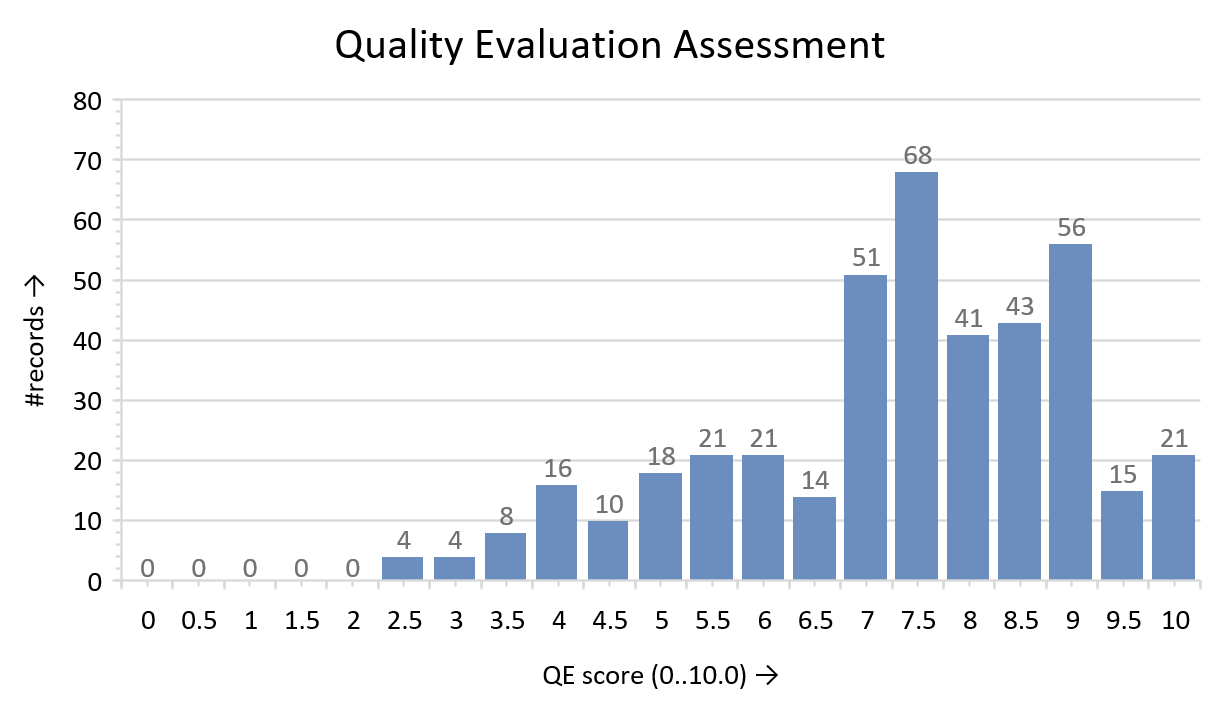
\includegraphics[width=\columnwidth]{figures/qe.png}%
  \label{fig:methodology:qe:qe}}
  \linebreak
  \subfloat[][]{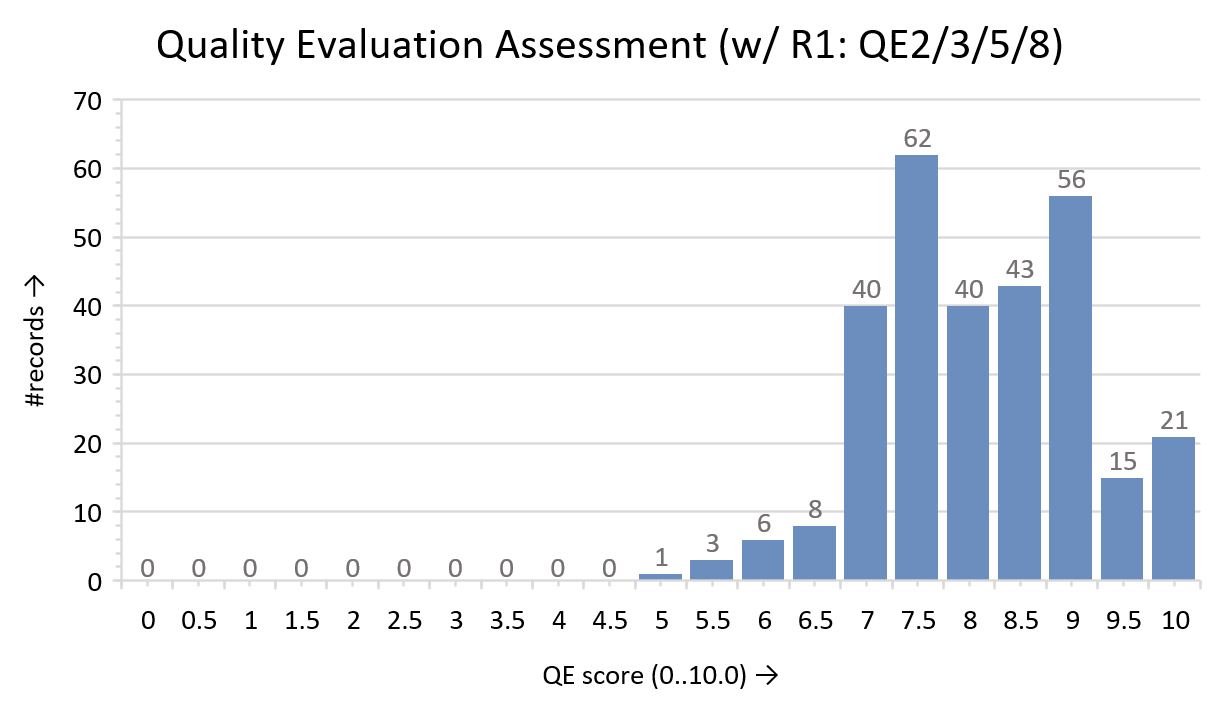
\includegraphics[width=\columnwidth]{figures/qe_wo-r1.png}%
  \label{fig:methodology:qe:qe_wo-r1}}
  \caption{Distribution of the quality evaluation scores obtained from assessing the eligible works considered in the review: (a) all eligible works; (b) works that pass the rejection criterion during the QE assessment related to QE2/3/5/8 = 0.0 (no compliance).}
  \label{fig:methodology:qe}
\end{figure}

The 8.5 cut-off score would not be suitable because methods that focus only on localization or mapping, or not having either the implementation or the experimental data publicly available would be obligated to have maximum scores in the other criteria to be included in the review. In these cases, a work would have a maximum score of 9.0 due to partial compliance on QE3 or no compliance on the QE7 criteria. Likewise, a cut-off score of 8.0 would only leave a margin for having a single partial compliance on QE1, QE2, QE4 or QE8 criteria in similar cases, even though it would reject 160/295 (54\%) records. Therefore, the 7.5/10.0 cut-off score is more appropriate for the quality assessment phase in this review by leaving margin for works to have partial compliance in more than one criterion. Indeed, this cut-off score allows an article with no public data and/or implementation (e.g., due to confidentiality agreements) to have up to four criteria with partial compliance, depending on the criterion's maximum score or if the work has available the experiments data and/or implementation. Another example is articles that only focus on localization or mapping. In these cases, the work could have no public implementation, even though requiring a maximum score on all other criteria, or, if the work has public data or implementation available, two other criteria could have partial compliance.

Overall, as illustrated in Figure~\ref{fig:methodology:prisma-flow}, the quality assessment of the 411 eligible works considering the two rejection criteria previously mentioned leads to rejecting a total of 236 (57\%) records. As a result, the remaining 175 records will be analyzed for data extraction.

\subsection{Data extraction}
\label{sec:methodology:data}

The data extraction process analyzes the records selected after the quality assessment phase and extracts information from these works. In the scope of this review, the Data Extraction (DE) items required for each record are the following ones:

\begin{itemize}[nosep]
\item $\left[\textbf{DE1}\right]$ \textbf{Long-term considerations} -- long-term factors the works consider in their proposed approach and experiments. Considering the knowledge obtained in the previous phases of this review's methodology, the authors considered the following factors for categorizing the included works:
  \begin{itemize}[nosep]
  \item appearance: varying conditions, appearance changes;
  \item dynamics: environment dynamics, dynamic elements;
  \item sparsity: map pruning, redundant data removal;
  \item multi-session: map management;
  \item computational: memory management, efficiency.
  \end{itemize}
\item $\left[\textbf{DE2}\right]$ \textbf{Localization} -- how the robot localizes itself and the type of localizer;
\item $\left[\textbf{DE3}\right]$ \textbf{Mapping} -- type of the map;
\item $\left[\textbf{DE4}\right]$ \textbf{Multi-robot} -- if the proposed methodologies consider multi-robot systems;
\item $\left[\textbf{DE5}\right]$ \textbf{Execution mode} -- offline, online, if requires both, or if no information on this item;
\item $\left[\textbf{DE6}\right]$ \textbf{Environment and domain} -- type of environment (indoor, outdoor) and domains (air, ground, water) tested with the proposed methodologies;
\item $\left[\textbf{DE7}\right]$ \textbf{Sensory setup} -- which sensors considered in the methodologies;
\item $\left[\textbf{DE8}\right]$ \textbf{Non-public experiments} -- if the authors performed experiments or tests with non-public data;
\item $\left[\textbf{DE9}\right]$ \textbf{Ground-truth} -- how ground-truth for non-public data is obtained or its type, if available;
\item $\left[\textbf{DE10}\right]$ \textbf{Distance and time characteristics} -- relative to the non-public experiments if available, as follows:
  \begin{itemize}[nosep]
  \item total distance (km) of the non-public experiments;
  \item path (km), in the case of repetitive paths;
  \item total time (h) in terms of continuous operation;
  \item time interval (day/week/month/year, or d/w/m/y) between the first and the last run.
  \end{itemize}
\item $\left[\textbf{DE11}\right]$ \textbf{Datasets} -- if and which public datasets are used in the experiments;
\item $\left[\textbf{DE12}\right]$ \textbf{Evaluation metrics} -- which metrics are used for evaluation.
\end{itemize}

In Section~\ref{sec:discussion:experiments}, a comparison table of the public datasets identified by the DE11 will contain the sensory setup, ground-truth data availability from the datasets, and the distance and time characteristics, similar to the data extraction items for non-public data, among other aspects. As a result, the distinction between public and non-public data availability represented in DE8, DE9, and DE10 allows to understand the distance and time characteristics of non-public data independently from the public datasets.

Although the data extraction phase in a systematic literature review usually does not remove any records, 33 of the analyzed 175 works have extended versions of the proposed methodologies, more detailed ones, or equivalent methods applied in different conditions.
Thus, these records are not included in the review to improve the discussion section in terms of singularity and originality of proposed approaches for the long-term localization and mapping problem.
The extracted information helped identifying the corresponding extended and more complete versions of these works.
A document containing the association of the removed versions to the records included in the review is available in the public GitHub repository, including their bibliographic references. 
Consequently, 142 original works are included in this review for an overview of these records in Section~\ref{sec:overview}, and their synthesis and discussion in Section~\ref{sec:discussion}. The information relative to the 12 data items for each of the included records is available in Appendix~\ref{a2:data-extraction} and also in the repository. The included works represent 34.55\% of the 411 eligible records for this review. This result indicates that the methodology followed in this review led to a high percentage of quality results.

